\documentclass[]{book}
\usepackage{lmodern}
\usepackage{amssymb,amsmath}
\usepackage{ifxetex,ifluatex}
\usepackage{fixltx2e} % provides \textsubscript
\ifnum 0\ifxetex 1\fi\ifluatex 1\fi=0 % if pdftex
  \usepackage[T1]{fontenc}
  \usepackage[utf8]{inputenc}
\else % if luatex or xelatex
  \ifxetex
    \usepackage{mathspec}
  \else
    \usepackage{fontspec}
  \fi
  \defaultfontfeatures{Ligatures=TeX,Scale=MatchLowercase}
\fi
% use upquote if available, for straight quotes in verbatim environments
\IfFileExists{upquote.sty}{\usepackage{upquote}}{}
% use microtype if available
\IfFileExists{microtype.sty}{%
\usepackage{microtype}
\UseMicrotypeSet[protrusion]{basicmath} % disable protrusion for tt fonts
}{}
\usepackage[a4paper]{geometry}
\usepackage{hyperref}
\PassOptionsToPackage{usenames,dvipsnames}{color} % color is loaded by hyperref
\hypersetup{unicode=true,
            pdftitle={Intermediate distance sampling workshop - St Andrews 2017},
            pdfauthor={Laura Marshall, David L. Miller and Len Thomas},
            colorlinks=true,
            linkcolor=blue,
            citecolor=Blue,
            urlcolor=Blue,
            breaklinks=true}
\urlstyle{same}  % don't use monospace font for urls
\usepackage{color}
\usepackage{fancyvrb}
\newcommand{\VerbBar}{|}
\newcommand{\VERB}{\Verb[commandchars=\\\{\}]}
\DefineVerbatimEnvironment{Highlighting}{Verbatim}{commandchars=\\\{\}}
% Add ',fontsize=\small' for more characters per line
\usepackage{framed}
\definecolor{shadecolor}{RGB}{248,248,248}
\newenvironment{Shaded}{\begin{snugshade}}{\end{snugshade}}
\newcommand{\KeywordTok}[1]{\textcolor[rgb]{0.13,0.29,0.53}{\textbf{#1}}}
\newcommand{\DataTypeTok}[1]{\textcolor[rgb]{0.13,0.29,0.53}{#1}}
\newcommand{\DecValTok}[1]{\textcolor[rgb]{0.00,0.00,0.81}{#1}}
\newcommand{\BaseNTok}[1]{\textcolor[rgb]{0.00,0.00,0.81}{#1}}
\newcommand{\FloatTok}[1]{\textcolor[rgb]{0.00,0.00,0.81}{#1}}
\newcommand{\ConstantTok}[1]{\textcolor[rgb]{0.00,0.00,0.00}{#1}}
\newcommand{\CharTok}[1]{\textcolor[rgb]{0.31,0.60,0.02}{#1}}
\newcommand{\SpecialCharTok}[1]{\textcolor[rgb]{0.00,0.00,0.00}{#1}}
\newcommand{\StringTok}[1]{\textcolor[rgb]{0.31,0.60,0.02}{#1}}
\newcommand{\VerbatimStringTok}[1]{\textcolor[rgb]{0.31,0.60,0.02}{#1}}
\newcommand{\SpecialStringTok}[1]{\textcolor[rgb]{0.31,0.60,0.02}{#1}}
\newcommand{\ImportTok}[1]{#1}
\newcommand{\CommentTok}[1]{\textcolor[rgb]{0.56,0.35,0.01}{\textit{#1}}}
\newcommand{\DocumentationTok}[1]{\textcolor[rgb]{0.56,0.35,0.01}{\textbf{\textit{#1}}}}
\newcommand{\AnnotationTok}[1]{\textcolor[rgb]{0.56,0.35,0.01}{\textbf{\textit{#1}}}}
\newcommand{\CommentVarTok}[1]{\textcolor[rgb]{0.56,0.35,0.01}{\textbf{\textit{#1}}}}
\newcommand{\OtherTok}[1]{\textcolor[rgb]{0.56,0.35,0.01}{#1}}
\newcommand{\FunctionTok}[1]{\textcolor[rgb]{0.00,0.00,0.00}{#1}}
\newcommand{\VariableTok}[1]{\textcolor[rgb]{0.00,0.00,0.00}{#1}}
\newcommand{\ControlFlowTok}[1]{\textcolor[rgb]{0.13,0.29,0.53}{\textbf{#1}}}
\newcommand{\OperatorTok}[1]{\textcolor[rgb]{0.81,0.36,0.00}{\textbf{#1}}}
\newcommand{\BuiltInTok}[1]{#1}
\newcommand{\ExtensionTok}[1]{#1}
\newcommand{\PreprocessorTok}[1]{\textcolor[rgb]{0.56,0.35,0.01}{\textit{#1}}}
\newcommand{\AttributeTok}[1]{\textcolor[rgb]{0.77,0.63,0.00}{#1}}
\newcommand{\RegionMarkerTok}[1]{#1}
\newcommand{\InformationTok}[1]{\textcolor[rgb]{0.56,0.35,0.01}{\textbf{\textit{#1}}}}
\newcommand{\WarningTok}[1]{\textcolor[rgb]{0.56,0.35,0.01}{\textbf{\textit{#1}}}}
\newcommand{\AlertTok}[1]{\textcolor[rgb]{0.94,0.16,0.16}{#1}}
\newcommand{\ErrorTok}[1]{\textcolor[rgb]{0.64,0.00,0.00}{\textbf{#1}}}
\newcommand{\NormalTok}[1]{#1}
\usepackage{longtable,booktabs}
\usepackage{graphicx,grffile}
\makeatletter
\def\maxwidth{\ifdim\Gin@nat@width>\linewidth\linewidth\else\Gin@nat@width\fi}
\def\maxheight{\ifdim\Gin@nat@height>\textheight\textheight\else\Gin@nat@height\fi}
\makeatother
% Scale images if necessary, so that they will not overflow the page
% margins by default, and it is still possible to overwrite the defaults
% using explicit options in \includegraphics[width, height, ...]{}
\setkeys{Gin}{width=\maxwidth,height=\maxheight,keepaspectratio}
\IfFileExists{parskip.sty}{%
\usepackage{parskip}
}{% else
\setlength{\parindent}{0pt}
\setlength{\parskip}{6pt plus 2pt minus 1pt}
}
\setlength{\emergencystretch}{3em}  % prevent overfull lines
\providecommand{\tightlist}{%
  \setlength{\itemsep}{0pt}\setlength{\parskip}{0pt}}
\setcounter{secnumdepth}{5}
% Redefines (sub)paragraphs to behave more like sections
\ifx\paragraph\undefined\else
\let\oldparagraph\paragraph
\renewcommand{\paragraph}[1]{\oldparagraph{#1}\mbox{}}
\fi
\ifx\subparagraph\undefined\else
\let\oldsubparagraph\subparagraph
\renewcommand{\subparagraph}[1]{\oldsubparagraph{#1}\mbox{}}
\fi

%%% Use protect on footnotes to avoid problems with footnotes in titles
\let\rmarkdownfootnote\footnote%
\def\footnote{\protect\rmarkdownfootnote}

%%% Change title format to be more compact
\usepackage{titling}

% Create subtitle command for use in maketitle
\newcommand{\subtitle}[1]{
  \posttitle{
    \begin{center}\large#1\end{center}
    }
}

\setlength{\droptitle}{-2em}
  \title{Intermediate distance sampling workshop - St Andrews 2017}
  \pretitle{\vspace{\droptitle}\centering\huge}
  \posttitle{\par}
  \author{Laura Marshall, David L. Miller and Len Thomas}
  \preauthor{\centering\large\emph}
  \postauthor{\par}
  \predate{\centering\large\emph}
  \postdate{\par}
  \date{2017-07-21}

\usepackage[scaled=0.95]{helvet}
\usepackage[T1]{fontenc}
\renewcommand{\familydefault}{\sfdefault}

\usepackage{amsthm}
\newtheorem{theorem}{Theorem}[chapter]
\newtheorem{lemma}{Lemma}[chapter]
\theoremstyle{definition}
\newtheorem{definition}{Definition}[chapter]
\newtheorem{corollary}{Corollary}[chapter]
\newtheorem{proposition}{Proposition}[chapter]
\theoremstyle{definition}
\newtheorem{example}{Example}[chapter]
\theoremstyle{remark}
\newtheorem*{remark}{Remark}
\begin{document}
\maketitle

{
\hypersetup{linkcolor=black}
\setcounter{tocdepth}{1}
\tableofcontents
}
\chapter*{Preface}\label{preface}
\addcontentsline{toc}{chapter}{Preface}

\chapter{A hands on introduction to R
tutorial}\label{a-hands-on-introduction-to-r-tutorial}

\chapter{analyse simulated data set}\label{analyse-simulated-data-set}

\chapter{Problem datasets}\label{problem-datasets}

\chapter{Creating distance sampling simulations using
DSsim}\label{creating-distance-sampling-simulations-using-dssim}

If you prefer to perform simulations using Distance 7.1, please skip
ahead to the section
\protect\hyperlink{running-distance-sampling-simulations-using-distance-7.1}{Running
distance sampling simulations using Distance 7.1} below.

\section{Aim}\label{aim}

The aim of this exercise is to run simulations which will allow you to
compare three different survey designs for a specific population. You
should judge these designs on their accuracy and precision.

You will also need the following R packages installed on your machine:
\texttt{DSsim}, \texttt{shapefiles}, \texttt{splancs} and \texttt{mrds}.
Now examine the other files and folders in the ``DSsim Exercise''
folder. There are three files starting with the name ``Region'' and
ending with .dbf, .shp and .shx, these files make up the shapefile for
the survey region. The ``density.surface.robj'' file is the density
surface for the survey region. The ``Survey Transects'' folder contains
a folder for each of the designs you are asked to look at, these contain
the transect shapefiles. The ``Results'' folder contains the results
from 999 replications as this can take a good few hours to run. To setup
the workspace first load the packages \texttt{DSsim} and
\texttt{shapefiles}, loading these two will automatically make
\texttt{splancs} and \texttt{mrds} available.

\begin{Shaded}
\begin{Highlighting}[]
\KeywordTok{library}\NormalTok{(DSsim)}
\KeywordTok{library}\NormalTok{(shapefiles)}
\end{Highlighting}
\end{Shaded}

\section{Create a region object}\label{create-a-region-object}

Read the Region shapefile into R using the \texttt{read.shapefile()}
function from the \texttt{shapefiles} package.

\begin{Shaded}
\begin{Highlighting}[]
\NormalTok{region.shapefile <-}\StringTok{ }\KeywordTok{read.shapefile}\NormalTok{(}\StringTok{"Region"}\NormalTok{)}
\end{Highlighting}
\end{Shaded}

Next you are going to create the region object using this shapefile. As
there are no strata you only need to provide a name for your survey
region and the units which are in metres (m). The survey region is
displayed in Figure \ref{fig:finishreg}.

\begin{Shaded}
\begin{Highlighting}[]
\NormalTok{region <-}\StringTok{ }\KeywordTok{make.region}\NormalTok{(}\DataTypeTok{region.name =} \StringTok{"Survey Region"}\NormalTok{, }\DataTypeTok{units =} \StringTok{"m"}\NormalTok{, }
                      \DataTypeTok{shapefile =}\NormalTok{ region.shapefile)}
\KeywordTok{plot}\NormalTok{(region, }\DataTypeTok{plot.units =} \StringTok{"km"}\NormalTok{)}
\end{Highlighting}
\end{Shaded}

\begin{figure}
\centering
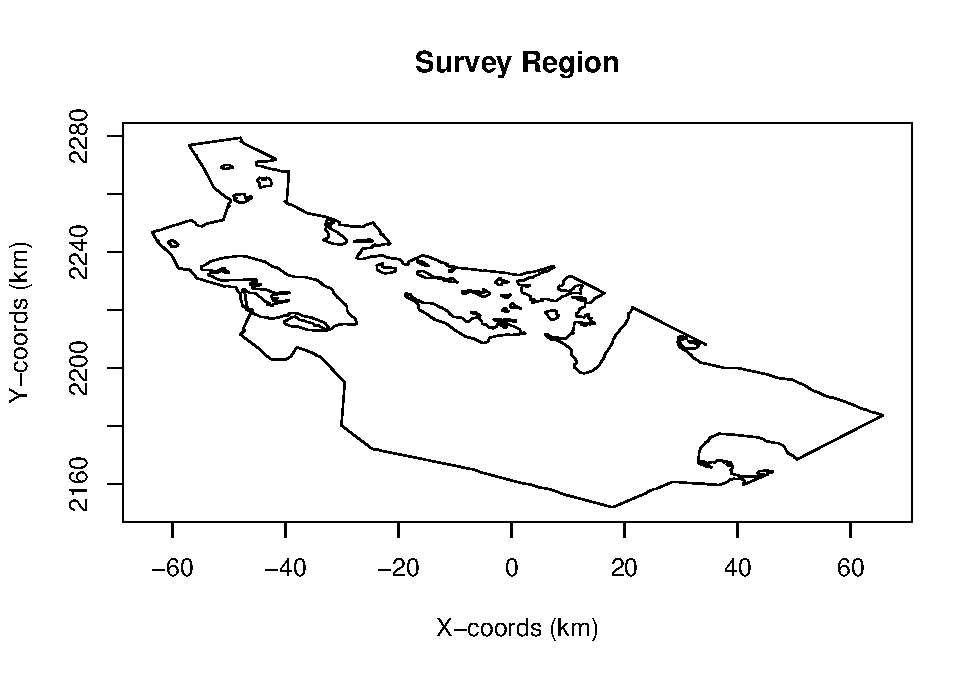
\includegraphics{_main_files/figure-latex/finishreg-1.pdf}
\caption{\label{fig:finishreg}Study region for simulation}
\end{figure}

\section{Create a density object}\label{create-a-density-object}

You are now going to create a density object within this region. For the
purposes of this exercise a density surface has already been created and
can be loaded as follows:

\begin{Shaded}
\begin{Highlighting}[]
\KeywordTok{load}\NormalTok{(}\StringTok{"density.surface.robj"}\NormalTok{)}
\end{Highlighting}
\end{Shaded}

You will see that an object called \texttt{density.surface} has appeared
in the workspace. This object is a list with one element (if the region
had been divided up into strata then this list would contain an element
for each strata). To have a look at what the density surface data look
like type \texttt{head(density.surface{[}{[}1{]}{]})}. You can see that
it is a data set of x and y locations and the densities at each point.

To create the density object you will need to provide the density
surface, the region object for which it was created and the grid spacing
that was used. I used a grid spacing of 1000m in both the x and y
directions to create this density surface. The density surface
describing animal distribution is shown in Figure 4.2.

\begin{Shaded}
\begin{Highlighting}[]
\NormalTok{pop.density <-}\StringTok{ }\KeywordTok{make.density}\NormalTok{(}\DataTypeTok{region =}\NormalTok{ region, }\DataTypeTok{density.surface =}\NormalTok{ density.surface, }
                            \DataTypeTok{x.space =} \DecValTok{1000}\NormalTok{, }\DataTypeTok{y.space =} \DecValTok{1000}\NormalTok{) }
\KeywordTok{plot}\NormalTok{(pop.density, }\DataTypeTok{plot.units =} \StringTok{"km"}\NormalTok{)}
\KeywordTok{plot}\NormalTok{(region, }\DataTypeTok{add =} \OtherTok{TRUE}\NormalTok{)}
\end{Highlighting}
\end{Shaded}

\begin{figure}
\centering
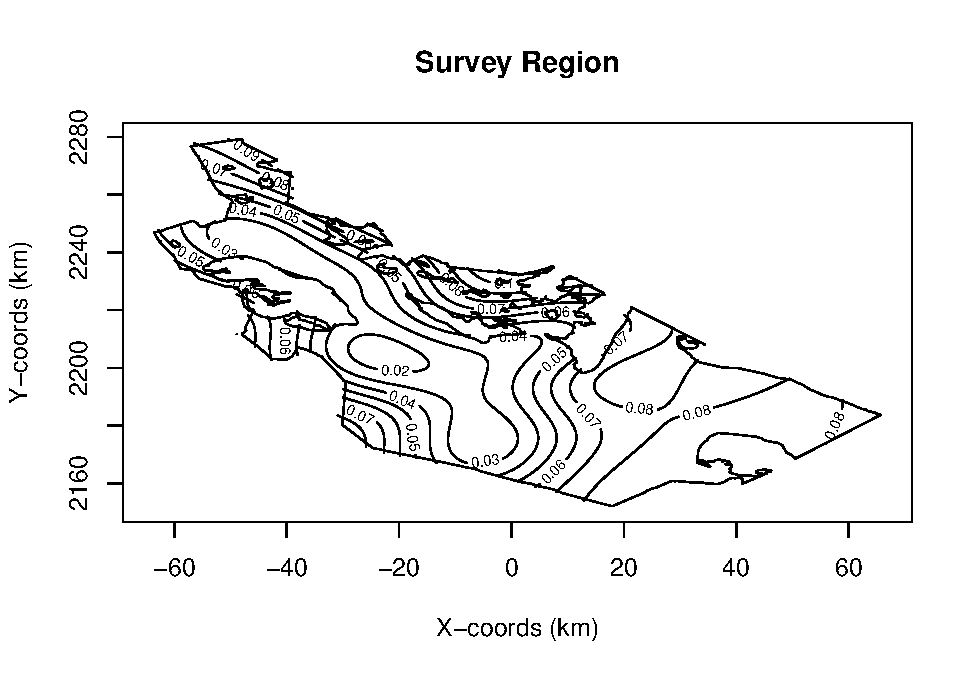
\includegraphics{_main_files/figure-latex/popden-1.pdf}
\caption{\label{fig:popden}Study region with animal density superimposed
Note lower density near the trail system}
\end{figure}

Optionally, the following code can be used to define your own density
surface. Firstly the density object is created with a constant value,
then high and low spots can be added with varying radii of influence.
The sigma parameter is used to calculate a Gaussian decay around the
central point.

\begin{Shaded}
\begin{Highlighting}[]
\NormalTok{alternative.density <-}\StringTok{ }\KeywordTok{make.density}\NormalTok{(}\DataTypeTok{region =}\NormalTok{ region, }\DataTypeTok{x.space =} \DecValTok{1000}\NormalTok{, }
                                    \DataTypeTok{y.space =} \DecValTok{1000}\NormalTok{, }\DataTypeTok{constant =} \FloatTok{0.4e-7}\NormalTok{)}

\NormalTok{alternative.density <-}\StringTok{ }\KeywordTok{add.hotspot}\NormalTok{(alternative.density, }\DataTypeTok{centre =} \KeywordTok{c}\NormalTok{(}\OperatorTok{-}\DecValTok{2500}\NormalTok{, }\DecValTok{2224000}\NormalTok{), }
                                   \DataTypeTok{sigma =} \DecValTok{10000}\NormalTok{, }\DataTypeTok{amplitude =} \FloatTok{0.1e-7}\NormalTok{)}
\NormalTok{alternative.density <-}\StringTok{ }\KeywordTok{add.hotspot}\NormalTok{(alternative.density, }\DataTypeTok{centre =} \KeywordTok{c}\NormalTok{(}\DecValTok{0}\NormalTok{, }\DecValTok{2184000}\NormalTok{), }
                                   \DataTypeTok{sigma =} \DecValTok{18000}\NormalTok{, }\DataTypeTok{amplitude =} \OperatorTok{-}\FloatTok{0.5e-8}\NormalTok{)}
\end{Highlighting}
\end{Shaded}

\section{Creating population description and detectability
objects}\label{creating-population-description-and-detectability-objects}

For this exercise we will fix the population size at 1500 individuals.
To do this set N = 1500 and tell it to generate exactly this number of
individuals (fixed.N = TRUE).

\begin{Shaded}
\begin{Highlighting}[]
\NormalTok{pop.description <-}\StringTok{ }\KeywordTok{make.population.description}\NormalTok{(}\DataTypeTok{region.obj =}\NormalTok{ region, }
                                               \DataTypeTok{density.obj =}\NormalTok{ pop.density, }
                                               \DataTypeTok{N =} \DecValTok{1500}\NormalTok{, }\DataTypeTok{fixed.N =} \OtherTok{TRUE}\NormalTok{)}
\end{Highlighting}
\end{Shaded}

We will now describe the detectability of the population using a
half-normal function with a sigma (scale.param) of 500m and a truncation
distance of 1000m. This means that around 2/3 of the detections will be
made within 500m of the transect and we will exclude anything sighted
further than 1000m perpendicular distance from the transect.

\begin{Shaded}
\begin{Highlighting}[]
\NormalTok{detect <-}\StringTok{ }\KeywordTok{make.detectability}\NormalTok{(}\DataTypeTok{key.function =} \StringTok{"hn"}\NormalTok{, }\DataTypeTok{scale.param =} \DecValTok{500}\NormalTok{, }\DataTypeTok{truncation =} \DecValTok{1000}\NormalTok{)}
\end{Highlighting}
\end{Shaded}

\section{Creating the survey design
object}\label{creating-the-survey-design-object}

We will now create a design object. For now concentrate on the
subjective design, we will come back to the parallel and zigzag designs
later. The subjective design was based on using some \textbf{existing
paths} to make the survey easier to carry out. Additional transects were
then added to achieve a more even coverage of the survey region.

NOTE: The path argument to describe where the files are located must
match your previous settings add ``/Survey Transects/Subjective
Design''.

\begin{Shaded}
\begin{Highlighting}[]
\NormalTok{subjective.design <-}\StringTok{ }\KeywordTok{make.design}\NormalTok{(}\DataTypeTok{transect.type =} \StringTok{"Line"}\NormalTok{, }
                                 \DataTypeTok{design.details =} \KeywordTok{c}\NormalTok{(}\StringTok{"user specified"}\NormalTok{), }
                                 \DataTypeTok{region =}\NormalTok{ region, }
                                 \DataTypeTok{plus.sampling =} \OtherTok{FALSE}\NormalTok{, }
                                 \DataTypeTok{path =} \StringTok{"Survey Transects/Subjective Design"}\NormalTok{)}
\end{Highlighting}
\end{Shaded}

\section{Creating the analyses
object}\label{creating-the-analyses-object}

The final thing we need to do before creating the simulation object is
describe the analyses we wish to carry out on the simulated data. Let's
try letting it choose between a half-normal and a hazard rate model
based on the AIC values.

\begin{Shaded}
\begin{Highlighting}[]
\NormalTok{ddf.analyses <-}\StringTok{ }\KeywordTok{make.ddf.analysis.list}\NormalTok{(}
                \DataTypeTok{dsmodel =} \KeywordTok{list}\NormalTok{(}\OperatorTok{~}\KeywordTok{cds}\NormalTok{(}\DataTypeTok{key =} \StringTok{"hn"}\NormalTok{, }\DataTypeTok{formula =} \OperatorTok{~}\DecValTok{1}\NormalTok{), }\CommentTok{#half-normal model}
                               \OperatorTok{~}\KeywordTok{cds}\NormalTok{(}\DataTypeTok{key =} \StringTok{"hr"}\NormalTok{, }\DataTypeTok{formula =} \OperatorTok{~}\DecValTok{1}\NormalTok{)),  }\CommentTok{#hazard rate model}
                \DataTypeTok{method =} \StringTok{"ds"}\NormalTok{, }\DataTypeTok{criteria =} \StringTok{"AIC"}\NormalTok{, }\DataTypeTok{truncation =} \DecValTok{1000}\NormalTok{)}
\end{Highlighting}
\end{Shaded}

\section{Creating the simulation
object}\label{creating-the-simulation-object}

We can finally put it all together and have a look at some example
populations, transects and survey data. I suggest you set the number of
repetitions (reps) to be fairly low or else it will take a long time to
run. For the subjective design you need to specify that it will be using
the same set of transects each time, single.transect.set = TRUE.

\begin{Shaded}
\begin{Highlighting}[]
\NormalTok{my.simulation.subjective <-}\StringTok{ }\KeywordTok{make.simulation}\NormalTok{(}\DataTypeTok{reps =} \DecValTok{10}\NormalTok{, }
                                            \DataTypeTok{single.transect.set =} \OtherTok{TRUE}\NormalTok{, }
                                            \DataTypeTok{region.obj =}\NormalTok{ region, }
                                            \DataTypeTok{design.obj =}\NormalTok{ subjective.design, }
                                            \DataTypeTok{population.description.obj =}\NormalTok{ pop.description,}
                                            \DataTypeTok{detectability.obj =}\NormalTok{ detect, }
                                            \DataTypeTok{ddf.analyses.list =}\NormalTok{ ddf.analyses)}
\end{Highlighting}
\end{Shaded}

Before running the simulation it is a good idea to have a check to see
that it is doing what you want. The function \texttt{check.sim.setup()}
will allow you to investigate the simulation properties. Having created
a population, transects, survey and detections, the function plots them
to assure you are happy with the simulation structure.

Let's check our subjective design simulation, see Figure
\ref{fig:plotsimul}.

\begin{Shaded}
\begin{Highlighting}[]
\KeywordTok{check.sim.setup}\NormalTok{(my.simulation.subjective)}
\end{Highlighting}
\end{Shaded}

\begin{figure}
\centering
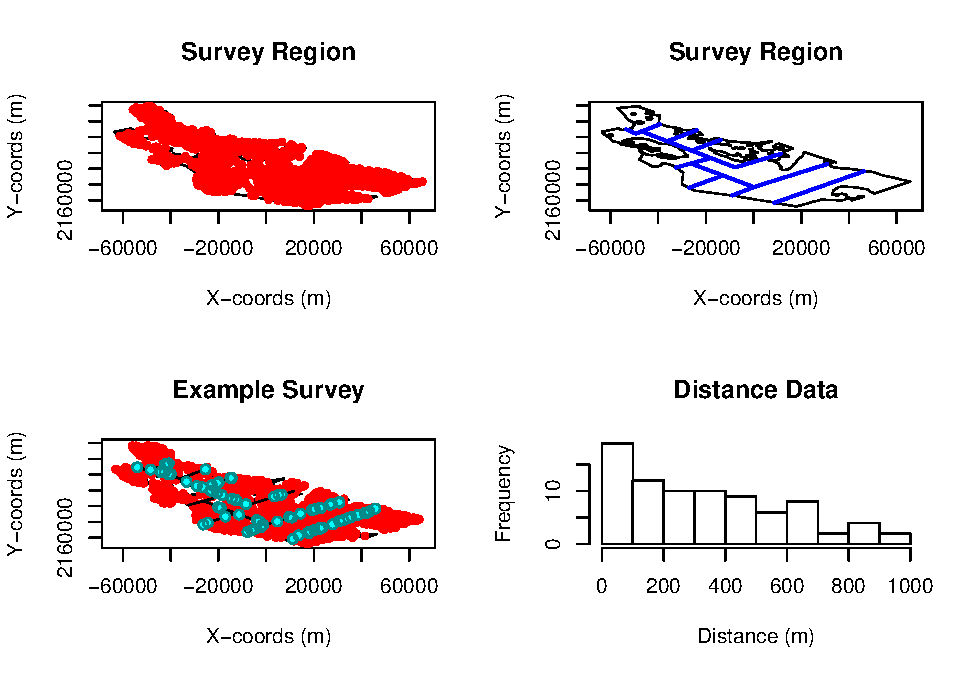
\includegraphics{_main_files/figure-latex/plotsimul-1.pdf}
\caption{\label{fig:plotsimul}Region, population, transects, detections}
\end{figure}

Once you are happy it is time to run the simulation. Please be patient
as it will take a few minutes to complete.

\begin{Shaded}
\begin{Highlighting}[]
\NormalTok{my.simulation.subjective  <-}\StringTok{ }\KeywordTok{run}\NormalTok{(my.simulation.subjective)}
\KeywordTok{summary}\NormalTok{(my.simulation.subjective, }\DataTypeTok{description.summary =} \OtherTok{FALSE}\NormalTok{)}
\end{Highlighting}
\end{Shaded}

\section{Now for the automated designs: Parallel
lines}\label{now-for-the-automated-designs-parallel-lines}

You will need to create a new simulation each with a new design object
for the parallel design. The other objects (region, density, population
description etc.) should be left the same.

NOTE: We now wish different transects to be used on each repetition
(\texttt{single.transect.set\ =\ FALSE}).

\begin{Shaded}
\begin{Highlighting}[]
\NormalTok{parallel.design <-}\StringTok{ }\KeywordTok{make.design}\NormalTok{(}\DataTypeTok{transect.type =} \StringTok{"Line"}\NormalTok{,}
                               \DataTypeTok{design.details =} \KeywordTok{c}\NormalTok{(}\StringTok{"Parallel"}\NormalTok{,}\StringTok{"Systematic"}\NormalTok{),}
                               \DataTypeTok{region.obj =}\NormalTok{ region, }\DataTypeTok{design.axis =} \DecValTok{45}\NormalTok{,}
                               \DataTypeTok{spacing =} \DecValTok{12000}\NormalTok{, }\DataTypeTok{plus.sampling =} \OtherTok{FALSE}\NormalTok{,}
                               \DataTypeTok{path =} \StringTok{"Survey Transects/Parallel Design"}\NormalTok{)}

\NormalTok{my.simulation.parallel <-}\StringTok{ }\KeywordTok{make.simulation}\NormalTok{(}\DataTypeTok{reps =} \DecValTok{10}\NormalTok{, }
                                          \DataTypeTok{single.transect.set =} \OtherTok{FALSE}\NormalTok{, }
                                          \DataTypeTok{region.obj =}\NormalTok{ region, }
                                          \DataTypeTok{design.obj =}\NormalTok{ parallel.design, }
                                          \DataTypeTok{population.description.obj =}\NormalTok{ pop.description,}
                                          \DataTypeTok{detectability.obj =}\NormalTok{ detect,}
                                          \DataTypeTok{ddf.analyses.list =}\NormalTok{ ddf.analyses)}
\end{Highlighting}
\end{Shaded}

Having created the features of the simulation, we want to check features
of the simulation have been correctly specified, see Figure
\ref{fig:parallelcheck}.

\begin{Shaded}
\begin{Highlighting}[]
\KeywordTok{check.sim.setup}\NormalTok{(my.simulation.parallel)}
\end{Highlighting}
\end{Shaded}

\begin{figure}
\centering
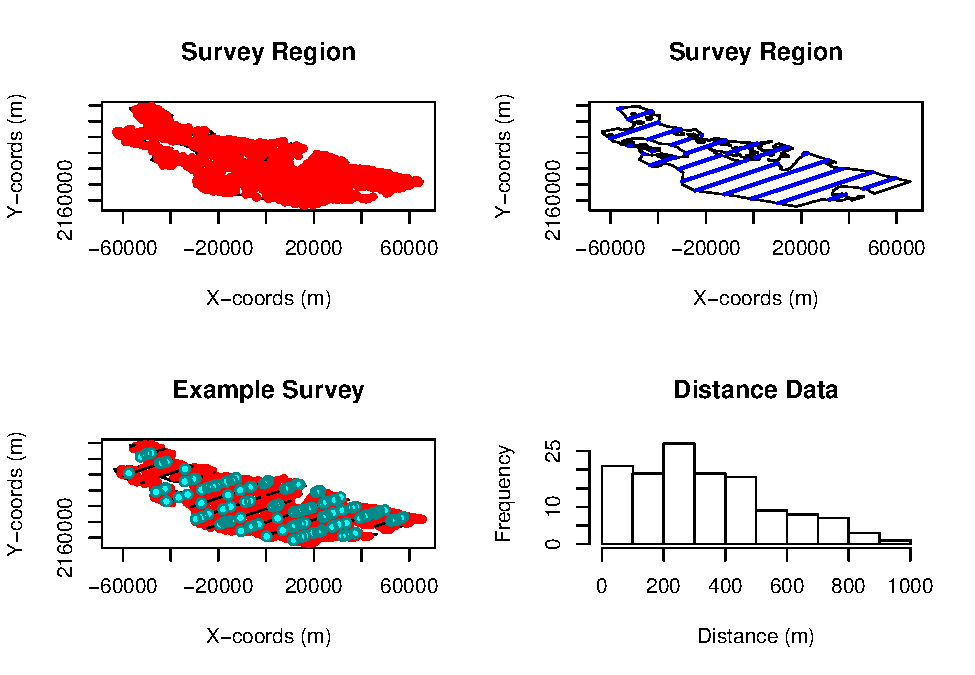
\includegraphics{_main_files/figure-latex/parallelcheck-1.pdf}
\caption{\label{fig:parallelcheck}Check setup of parallel transect design
simulation}
\end{figure}

When satisfied with this simulation setup, you would proceed to run your
parallel design simulation.

\begin{Shaded}
\begin{Highlighting}[]
\NormalTok{my.simulation.parallel  <-}\StringTok{ }\KeywordTok{run}\NormalTok{(my.simulation.parallel)}
\KeywordTok{summary}\NormalTok{(my.simulation.parallel, }\DataTypeTok{description.summary =} \OtherTok{FALSE}\NormalTok{)}
\end{Highlighting}
\end{Shaded}

\subsection{ZigZag survey design}\label{zigzag-survey-design}

Now have a go at creating and running a simulation using the equal
spaced zigzag design transects in the ``Zigzag Design'' folder. The
spacing used to generate these was 8250m on a design axis of 135
degrees. Use \texttt{?make.design} for help.

Having created the features of the simulation, check the features of the
simulation have been correctly specified (Fig. \ref{fig:zigzagcheck}).

\begin{figure}
\centering
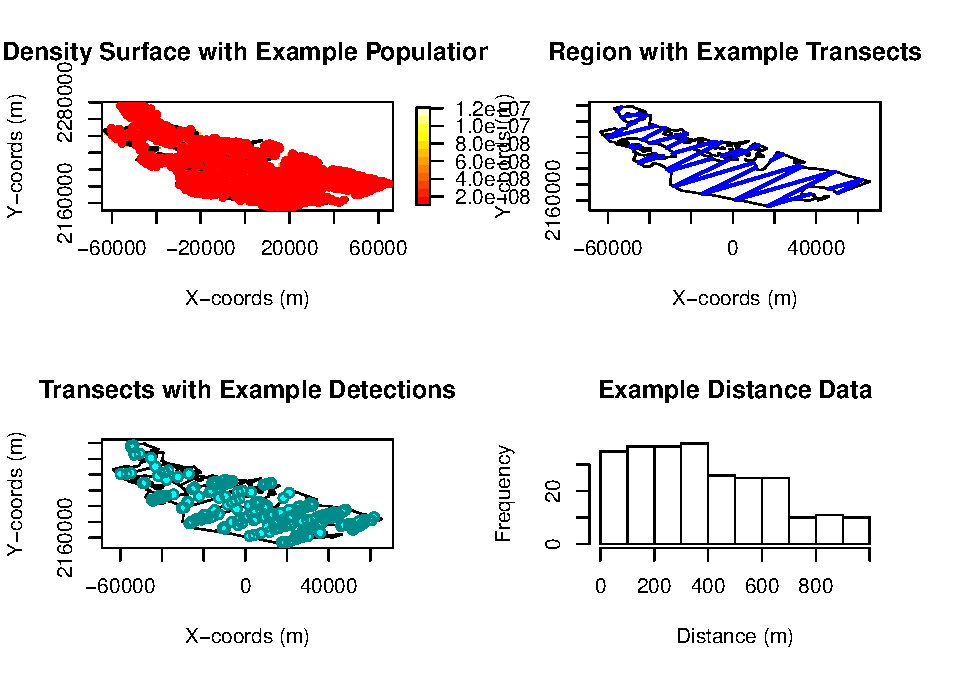
\includegraphics{_main_files/figure-latex/zigzagcheck-1.pdf}
\caption{\label{fig:zigzagcheck}Check setup of zigzag transect design
simulation}
\end{figure}

When satisfied with this simulation setup, you would proceed to run your
zigzag design simulation.

\begin{Shaded}
\begin{Highlighting}[]
\NormalTok{my.simulation.zigzag  <-}\StringTok{ }\KeywordTok{run}\NormalTok{(my.simulation.zigzag)}
\KeywordTok{summary}\NormalTok{(my.simulation.zigzag)}
\end{Highlighting}
\end{Shaded}

\section{Results from 999
repetitions}\label{results-from-999-repetitions}

I ran each of these simulations 999 times and stored the simulations as
R objects. Load these into the R workspace using the following code:

\begin{Shaded}
\begin{Highlighting}[]
\KeywordTok{load}\NormalTok{(}\StringTok{"Results/simulation.subjective.robj"}\NormalTok{)}
\KeywordTok{load}\NormalTok{(}\StringTok{"Results/simulation.parallel.robj"}\NormalTok{)}
\KeywordTok{load}\NormalTok{(}\StringTok{"Results/simulation.zigzag.robj"}\NormalTok{)}
\end{Highlighting}
\end{Shaded}

The objects \texttt{simulation.subjective}, \texttt{simulation.parallel}
and \texttt{simulation.zigzag} will now be in your workspace. Have a
look at the results using the \texttt{summary()} function and use them
to fill in the table below, Figure 4.5.

\begin{Shaded}
\begin{Highlighting}[]
\KeywordTok{summary}\NormalTok{(simulation.subjective)}
\KeywordTok{summary}\NormalTok{(simulation.parallel)}
\KeywordTok{summary}\NormalTok{(simulation.zigzag)}
\end{Highlighting}
\end{Shaded}

Which survey design would you recommend? Why?\\
What would happen if our assumptions about animal distribution were
incorrect?

\begin{figure}
\centering
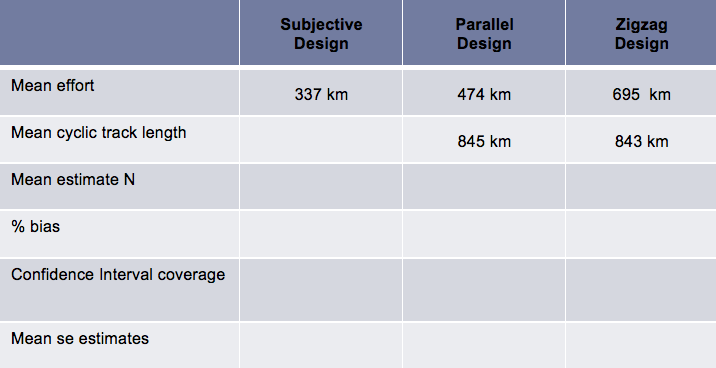
\includegraphics{images/results.png}
\caption{Results Table}
\end{figure}

\hypertarget{running-distance-sampling-simulations-using-distance-7.1}{\section{Running
distance sampling simulations using Distance
7.1}\label{running-distance-sampling-simulations-using-distance-7.1}}

If you would like to investigate different designs then these can be
created and used in simulations in Distance 7.1. Note that currently the
simulation options in Distance 7.1 are somewhat more restricted than in
DSsim.

We have created a Distance project based on the scenario just described
and setup the systematic parallel and equal spaced zigzag designs as
specified above. This project is named \texttt{DSsimExercise}. This
exercise will lead you through replicating the previous simulations in
Distance, but you could choose to invesgitate different designs or even
try out some simulations on your own study area if you prefer.

If you wish to try out simulations on your own study area help on
importing geographic data, creating designs and analyses can be found in
the Distance manual.

\section{Creating simulations in
Distance}\label{creating-simulations-in-distance}

\subsection{Simulation Details}\label{simulation-details}

Open the \texttt{DSsimExercise.dst} project and navigate to the
Simulation Browser tab (on the far right, with the rabbit coming out of
the hat). Now create a new simulation and give it a meaningful name.
Open the details for this simulation, Figure 4.6.

\begin{itemize}
\tightlist
\item
  Select the \textbf{design} option for these simulations as we want to
  use a different survey (set of transects) in each iteration and then
  select which design to use from the dropdown menu.

  \begin{itemize}
  \tightlist
  \item
    Distance will generate the required number of surveys for the
    simulation. (Selecting the \textbf{survey} option will instruct
    Distance to use only a single set of transects for the whole
    simulation.)\\
  \end{itemize}
\item
  Select a data filter with an absolute right truncation distance.

  \begin{itemize}
  \tightlist
  \item
    The truncation distance specified in the data filter will give the
    greatest perpendicular distance at which an observation can be made
    and the distance to which the detection function model(s) will be
    fitted.\\
  \end{itemize}
\item
  Select one or more (mrds) models to fit to the simulated data. Here we
  can use the MADS HN v HR model definition (ID 3) to point to both the
  half-normal and hazard rate model definitions.

  \begin{itemize}
  \tightlist
  \item
    Use the Properties button to have a look at the MADS model
    definition properties, particularly the detection function tab.
  \item
    The model with the minimum AIC will be selected in each simulation
    iteration.
  \end{itemize}
\end{itemize}

\begin{figure}
\centering
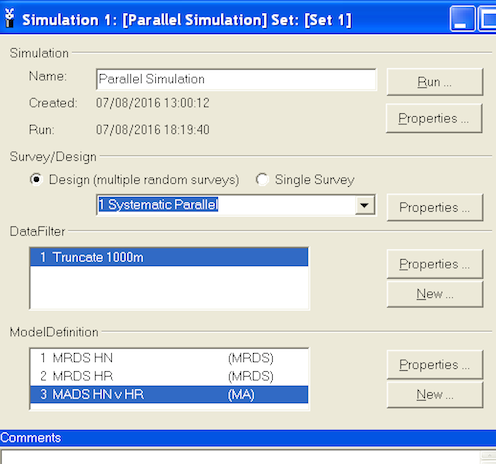
\includegraphics{images/details.png}
\caption{Simulation Details}
\end{figure}

\subsection{Simulation Properties}\label{simulation-properties}

Now click on the Simulation `Properties' button to set the other
simulation properties. The Simulation tab (Figure 4.7) allows us to
specify the geographic layer to use, in this example as we do not have
strata we must select the global study region layer. Here we can also
tell Distance how many times to repeat the simulation and set shapefile
options. It is sensible to run the simulation only once in the first
instance to check the setup is correct. The shapefile options allow us
to tell Distance to save the shapefiles for use in subseqent simulations
using the same design. This can save some processing time. If requested
the shapefiles are stored in the project .dat folder under
`Simulation/Simulation{[}ID{]}/shapefiles'.

\begin{figure}
\centering
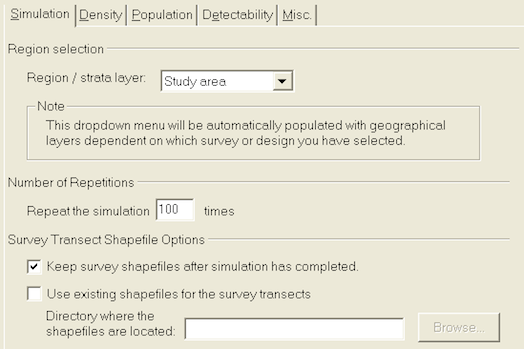
\includegraphics{images/simulation.png}
\caption{Properties Pages: Simulation tab}
\end{figure}

Next we can define our density surface which describes animal
distribution (Figure 4.8). As in exercise 1A we can select a grid
spacing of 1000. Distance has more restricted options than DSsim.
Currently we are only able to specify a constant density surface with
hot/low spots. Note that this density surface is just giving Distance
the relative (rather than absolute) densities.

\begin{figure}
\centering
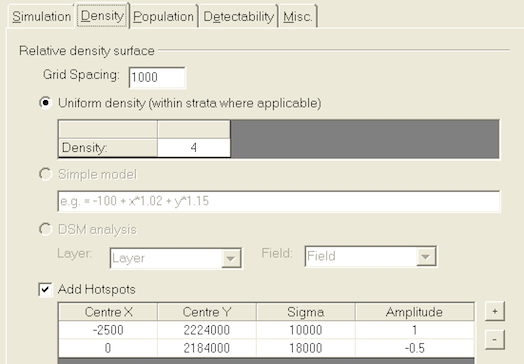
\includegraphics{images/density.png}
\caption{Properties Pages: Density tab}
\end{figure}

\newpage

The Population tab (Figure 4.9) currently only requires that we provide
a population size, in this case 1500.

\begin{figure}
\centering
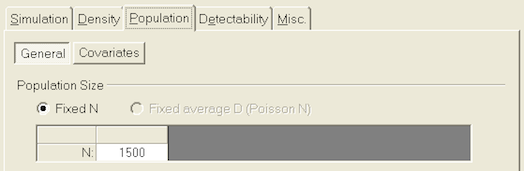
\includegraphics{images/population.png}
\caption{Properties Pages: Population tab}
\end{figure}

Next we describe the detectability of the animals. We will assume a
half-normal detection function with sigma = 500m (Figure 4.10). The
units of the detection function parameters must be the same as those of
the study region and a reminder is provided below the table.

\begin{figure}
\centering
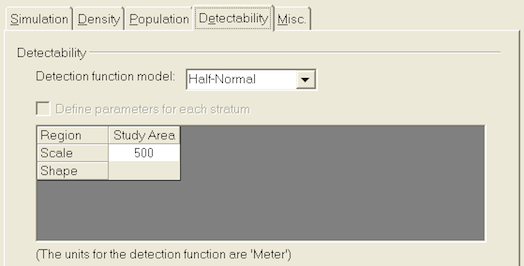
\includegraphics{images/detect.png}
\caption{Properties Pages: Detectability tab}
\end{figure}

Finally we can select some miscelaneous options. These do not affect the
output seen within distance. The option to run the simulation in
parallel can speed things up if running more than a few iterations.
Saving the results from each iteration to file will create csv files
with the individual estimates from each repetition. Saving an example
dataset will create a csv file that is ready to be read into a distance
project for analysis. These files are stored in the project .dat folder
under `Simulation/Simulation{[}ID{]}'.

Further instructions on setting up different simulations options can be
found in the Distance manual.

\subsection{Results}\label{results}

Solutions to this practical can be found in the
DSsimExerciseSolutions.dst project. In this project both the parallel
and zigzag design simulations have been run 100 times.

Note that even though the designs were never initially run to estimate
coverage, when a simulation is run this triggers the design to be run.
Therefore, the design results give the coverage for the actual sets of
transects used in the simulation.

\chapter{Preparing survey data for spatial
analysis}\label{preparing-survey-data-for-spatial-analysis}

\chapter{Detection function fitting}\label{detection-function-fitting}

\chapter{Simple density surface
models}\label{simple-density-surface-models}

\chapter{Advanced density surface
models}\label{advanced-density-surface-models}

\chapter{Prediction using fitted density surface
models}\label{prediction-using-fitted-density-surface-models}

\chapter{Estimating precision of predictions from density surface
models}\label{estimating-precision-of-predictions-from-density-surface-models}

\chapter{Mark-recapture distance sampling of
golftees}\label{mark-recapture-distance-sampling-of-golftees}

\chapter*{References}\label{references}
\addcontentsline{toc}{chapter}{References}


\end{document}
